\subsubsection{AASIST}
AASIST (\textit{Audio Anti-Spoofing using Integrated Spectro-Temporal Graph Attention Networks})  es un modelo creado con la motivación de combinar pistas espectrales y temporales para detectar artefactos de spoofing y conseguir robustez frente a una gran variedad de ataques.
Como este modelo produce una predicción a partir del audio crudo por lo que el primer paso es definir las rutas a los audios. 

Después, se lee el contenido del \textbf{archivo .conf} del modelo. Para ello, hemos creado una función que busca el elemento pasado por parámetro y devuelve el bloque superior que contiene ese elemento junto con los elementos al mismo nivel. Esto nos permite construir una variable, que vamos a llamar args, con los siguientes campos:
\begin{itemize}
    \item \textbf{first\_conv}: configuración del \textbf{kernel} de la primera capa de convolución, es decir, cuántas muestras de audio se utilizan para cada filtro. En este caso, 128.
    \item \textbf{filts}: es un array de elementos siendo el primero el número de \textbf{filtros} en la primera capa de convolución. Los siguientes elementos son pares para cada bloque residual con el número de filtros de entrada y de salida.
    \item \textbf{gat\_dims}: tamaño del \textbf{embedding} que representa cada nodo. Tiene dos valores que hacen referencia al tamaño al construir los grafos de atención y al tamaño en las fases de ``HS-GAL'' + ``pooling'' respectivamente.
    \item \textbf{pool\_ratios}: se usa en la técnica de ``graph pooling'' y significa el \textbf{ratio de reducción de nodos} en cada capa. Los dos primeros valores se usan para reducir los grafos espectral y temporal respectivamente antes de combinarlos en el grafo heterogéneo. El siguiente valore se usa para reducir el grafo heterogéneo después de cada capa HS-GAL. Aunque existe un cuarto valor, en el modelo final no se usa.
    \item \textbf{temperatures}: controla lo suave o agresiva que es la \textbf{atención} en cada fase. Cuanto más bajo es este parámetro, mayor peso se concentra en pocos nodos vecinos.
\end{itemize}
Con args ya creado, la usamos para instanciar el modelo. Posteriormente, se usa el checkpoint para cargar los pesos preentrenados. 

El siguiente paso es definir las funciones de inferencia. Para esto, nos apoyamos primero en dos funciones auxiliares, una que convierte los audios a un \textbf{formato estándar}, un solo canal y 16 kHz, y otra que crea una \textbf{ventana} para recorrer audios largos. Esta última es importante ya que AASIST está diseñado para recibir segmentos de longitud de unos 4 segundos.
Con esto preparado, las tres funciones de inferencia las creamos para ver si conseguiamos mejores resultados alterando un un poco el proceso y se describen a continuación:
\begin{itemize}
    \item \textbf{average\_windows}: esta función devuelve la media de sumar las predicciones de cada ventana calculadas de forma independiente. 
    \item \textbf{score\_without\_windows}: esta función devuelve solamente la puntuación del segmento incial del audio en archivos largos o del audio en su totalidad en el caso contrario.
    \item \textbf{average\_logits}: esta función fusiona todas las ventana sumando sus logits antes de calcular una única probabilidad.
\end{itemize}
Finalmente, se aplica el modelo y se vuelcan los resultados en un csv con el nombre del audio, la probabilidad de que sea ``bonafide'' y su duración. Para esto, se recorre cada audio del dataset, se le aplica una de las funciones de inferencia y se escribe la información en el csv.

\paragraph{Resultados y análisis}

Como hemos mencionado anteriormente, implementamos tres funciones de inferencia distintas para intentar obtener mejores resultados. Tras varias pruebas, alternando las tres funciones, obtuvimos resultados pésimos en los que el modelo tendía a clasificar cada muestra como “bona fide” y alguna como “spoof” pero sin mucho acierto lo que da una sensación de clasificación al azar.
Ante estos resultados, decidimos realizar fine-tunning sobre el propio modelo preentrenado, nuestro propio preentrenamiento con parte del dataset que creamos. Para conseguir esto, primero separamos el dataset en train, eval y dev y generamos los archivos de “protocols” de donde el modelo va leyendo el nombre y el tipo de los audios de cada partición. Adicionalmente, tuvimos que hacer ciertos ajustes en el .conf y en especial, ajustar el número de épocas.

Para las pruebas, las hemos separado en tres tipos: audios en inglés por separado, español por separado y ambos idiomas juntos. Dentro de cada escenario, hay cuatro pruebas con distinto número de \textbf{épocas: 10, 20, 40 o 80}. También, cabe mencionar que siempre se ha mantenido una proporción en la separación en train, dev y eval de 72\%, 14\% y 14\%, respectivamente. 
Por último, antes de analizar los resultados, es importante explicar que en la separación manual del dataset hemos separado los distintos speakers que había en cada idioma. Esto se refiere a que en el dataset hay por idioma, 5 speakers distintos con 10 audios “bonafide” y 10 “spoof, entonces, hemos intentado que en las tres particiones haya audios de las 5 personas y así intentar evitar sesgos.

A la hora de evaluar, hemos usado 3 medidas:

\textbf{Precision}: proporción de las muestras spoof detectadas sobre el total de muestras clasificadas como spoof 

 $\text{Precision}=\frac{TP}{TP+FP}$
\textbf{Recall}: proporción de muestras spoof detectadas correctamente sobre el total de muestras spoof

 $\text{Recall}=\frac{TP}{TP+FN}$

\textbf{F1}: media armónica entre precision y recall

 $\text{F1} = \frac{2\cdot \text{Precision}\cdot \text{Recall}}{\text{Precision}+\text{Recall}}$

\begin{figure}
	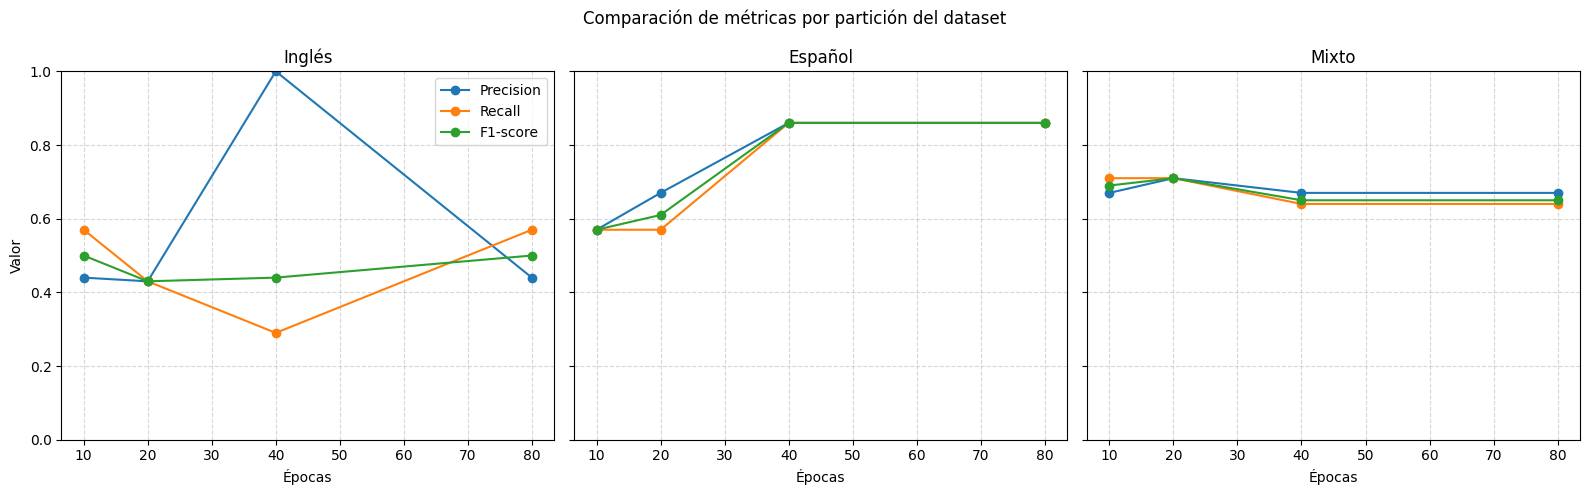
\includegraphics[width=\textwidth]{imagenes/AASIST_resultados_preentrenamientos.png}
	\caption{Resultados del preentrenamiento en AASIST.}
	\label{fig:voto_mayoria}
\end{figure}
Lo primero que podemos destacar sobre las gráficas, es que el modelo clasifica claramente mejor los audios en español ya que todas las métricas, a excepción de precisión en 40 épocas, tienen valores superiores. Esta diferencia explica el porqué la partición mixta lo hace peor que la que solo tiene muestras en inglés y permite deducir que ejecutar ambos idiomas juntos no le ayuda a clasificarlos mejor. 

En lo referido a las épocas, lo más destacable es que superar las 40 épocas empeora la predicción por lo que podemos suponer que está ocurriendo un fenómeno de sobreaprendizaje. También, podemos observar que en la partición en inglés, el aumento del valor de este parámetro no equivale en términos generales a una subida en la mejora de la predicción, fenómeno que no ocurre con la partición en español.



